%CaseQuad

Air traffic control (ATC) offers many opportunities for automation to allow a more efficient and safer landing patterns. The constraints of air traffic control are complex and contain many safety rules. In this example we express a simplified version these rules for an autonomous ATC for quad-rotors in MTL and demonstrate how the smoothed robustness is used to generate control strategies for safely and robustly landing two quadrotors in an enclosed airspace with an obstacle. Simulation results with three initial trajectories (for a multi-start) show that the proposed approach outperforms Simulated Annealing and gradient descent on the non-smooth robustness.

The specification for the autonomous ATC with two-quadrotors in the airspace is:
{\small
\begin{subequations}
\begin{align}
\Psi &= \eventually_{[0,N]}(p_1 \in \text{Terminal}) \land \eventually_{[0,N]}(p_2 \in \text{Terminal}) \land   \nonumber \\
& \always_{[0,N]} (\neg (p_1 \in \text{Zone}_1) \lor z_1 \in [1,5]) \land \nonumber \\
& \always_{[0,N]} (\neg (p_2 \in \text{Zone}_1) \lor z_2 \in [1,5]) \land \nonumber \\
& \always_{[0,N]} (\neg (p_1 \in \text{Zone}_2) \lor z_1 \in [0,3]) \land \nonumber \\
& \always_{[0,N]} (\neg (p_2 \in \text{Zone}_2) \lor z_2 \in [0,3]) \land \nonumber \\
& \always_{[0,N]} (\neg (p_1 \in \text{Unsafe})) \land \always_{[0,N]} (\neg (p_2 \in \text{Unsafe})) \land  \nonumber \\
& \always_{[0,N]} (||p_1-p_2||_2^2 \geq d_{min}^2)
\end{align}
\end{subequations}
}

Here $p_1$ and $p_2$ refer to the position of the two quad-rotors in $(x,y,z)$-space. The specification implies that, within a horizon of $N$ steps,  both quad-rotors should: a) eventually land (reach the terminal zone), b) Follow altitude rules in two zones, $\text{Zone}_1$ and $\text{Zone}_2$ which have different altitude ($z$) floors and ceilings, c) Avoid the $\text{Unsafe}$ set, and d) always maintain a safe distance between each other ($d_{min}$). Note, that unlike the previous example, turning the specification into constraints (possibly non-convex) for the control problem is no longer trivial. This is due to the $\eventually$ operator, which would require a MILP formulation to be accounted for. In addition, the minimum separation and altitude-rules for the two zones cannot be turned into convex constraints for the optimization. As will be seen below, our approach allows us to keep the non-convexity in the cost function, have convex (linear) constraints on the optimization problem.

The $\text{Airspace}$ here is a hyper-rectangle in $\mathbb{R}^3$, $[-5,5] \times [-5,5] \times [0,5]$, where $\times$ represents the Cartesian product. $\text{Zone}_1$, $[-5,0] \times [-5,5] \times [0,5]$, is the zone where the quad-rotors enter the $\text{Airspace}$ (i.e. where initial positions are), and has a ceiling of $5$ m and an enforced floor of $1$ m. Similarly, $\text{Zone}_2$, $[0,5] \times [-5,5] \times [0,5]$, is the zone where the $\text{Terminal}$ landing zone is, and it has a lower floor of $0$ m, and ceiling of $3$ m. The $\text{Terminal}$ set is a hyper-cube of length 1, given by $[3,4] \times [3,4] \times [0,1]$. Finally, the $\text{Unsafe}$ set is a hyper-rectangle $[-1,1] \times [-1,1] \times [0,5]$ in the middle of the air-space. In simulation, $d_{min}$ is set to $0.2$ m. The formula horizon $N$, is set to $20$.

This arrangement of the air-space, where the specifications for altitude ceiling and floors for either zone are in a $A \implies B$ (or $ \neg A \lor B$) format, is common in ATC and also allows us to combine the $\text{Airspace}$ with velocity-limits ($[-5,5]^3$) into the set $X$, which is a convex (Polyhedron) set constraint on the state of both quad-rotors, as will be explained below.

The quad-rotor dynamics are obtained via linearization around hover, and discretization at $5$-Hz. Similar models have been used for control of real quad-rotors with success (\cite{RTSS15}). For simulation, we set the mass of the either quad-rotor to be $0.5$ kg. Acceleration due to gravity is $9.8\,ms^{-1}$. The corresponding linearized and discretized quad-rotor dynamics are given as:

{\tiny
\begin{equation}
\begin{bmatrix} \dot{x}_{k+1} \\ \dot{y}_{k+1} \\ \dot{z}_{k+1} \\ x_{k+1} \\ y_{k+1} \\ z_{k+1} \end{bmatrix}= \begin{bmatrix} 1&0&0&0&0&0 \\0&1&0&0&0&0 \\0&0&1&0&0&0 \\0.2&0&0&1&0&0 \\0&0.2&0&0&1&0 \\0&0&0.2&0&0&1\end{bmatrix} \begin{bmatrix} \dot{x}_{k} \\ \dot{y}_{k} \\ \dot{z}_{k} \\ x_{k} \\ y_{k} \\ z_{k} \end{bmatrix} + \begin{bmatrix} 1.96&0&0 \\ 0&-1.96&0 \\0&0&0.4 \\0.196&0&0 \\0&-0.196&0\\0&0&0.04 \end{bmatrix} \begin{bmatrix} \theta_k \\ \phi_k \\ \text{T}_k \end{bmatrix}
\end{equation}
}

Here, the state consists of the velocities and positions in the $x,y,z$ co-ordinates. The inputs to the system are the desired roll angle $\theta$, pitch angle $\phi$ and thrust $\text{T}$. In a real quad-rotor, a high-frequency low-level controller (not simulated) is responsible for generating rotor speeds to match the desired roll, pitch and thrust (with yaw generally set to be stabilized at $0$). 

The control problem is to maximize the smooth robustness of the specification $\srob_{\Psi}$, subject to the dynamics of two identical quad-rotors, and input limits of $0.5236$ radians (or $30$ degrees) on both roll and pitch, and $\text{T}\in[-1.5,1.5]$, giving us the set $U$. The set $X$ for state limits on either quadrotor is, as defined earlier, the Cartesian product of velocity limits $[-5,5]^3$ and the $\text{Airspace}$ set, i.e. $[-5,5]^3$. Also with respect to the general control problem, \eqref{eq:general_ctrl}, we set $\gamma=0$ and $\delta=0$. This keeps the smooth robustness only in the cost (to be maximized) and allows a fair comparison of the optimization of robustness with other methods. In general, our formulation has linear constraints (dynamics and $X$, $U$) for both quad-rotors, allowing us to easily apply off the shelf optimization solvers.
 %, Simulated Annealing and gradient descent, via SQP, on the robustness function.

For simulation purposes, we use obtain 3 initial trajectories (via solving different linear programs) from the given initial state to the terminal (landing) set. These three trajectories, each of which has negative robustness (i.e. does not satisfy the given specification), serve as three different initial solutions to A) Our approach B) Gradient-descent via SQP, using the actual robustness function as the cost, C) Simulated Annealing with the actual robustness function as the cost. This multi-start approach can be used in practice when there is a fast initial trajectory generator available.

Fig.\ref{fig:quad_init} shows the initial trajectories for both the quadrotors in the given air-space, neither of which satisfy the specification $\Psi$. Fig.\ref{fig:quad_ssqp} shows the three trajectories obtained after applying our control method, with the three initial trajectories as starting points for the optimization, respectively. All three trajectories obtained satisfy the specification $\Psi$, showing the applicability of our method. To avoid clutter, we do not show trajectories obtained from the other two methods, but summarize the results in a table. Table shows for the three trajectories, initial robustness, robustness for trajectory obtained via the three methods (and the approximate robustness when applicable).

\begin{figure}[t]
\centering
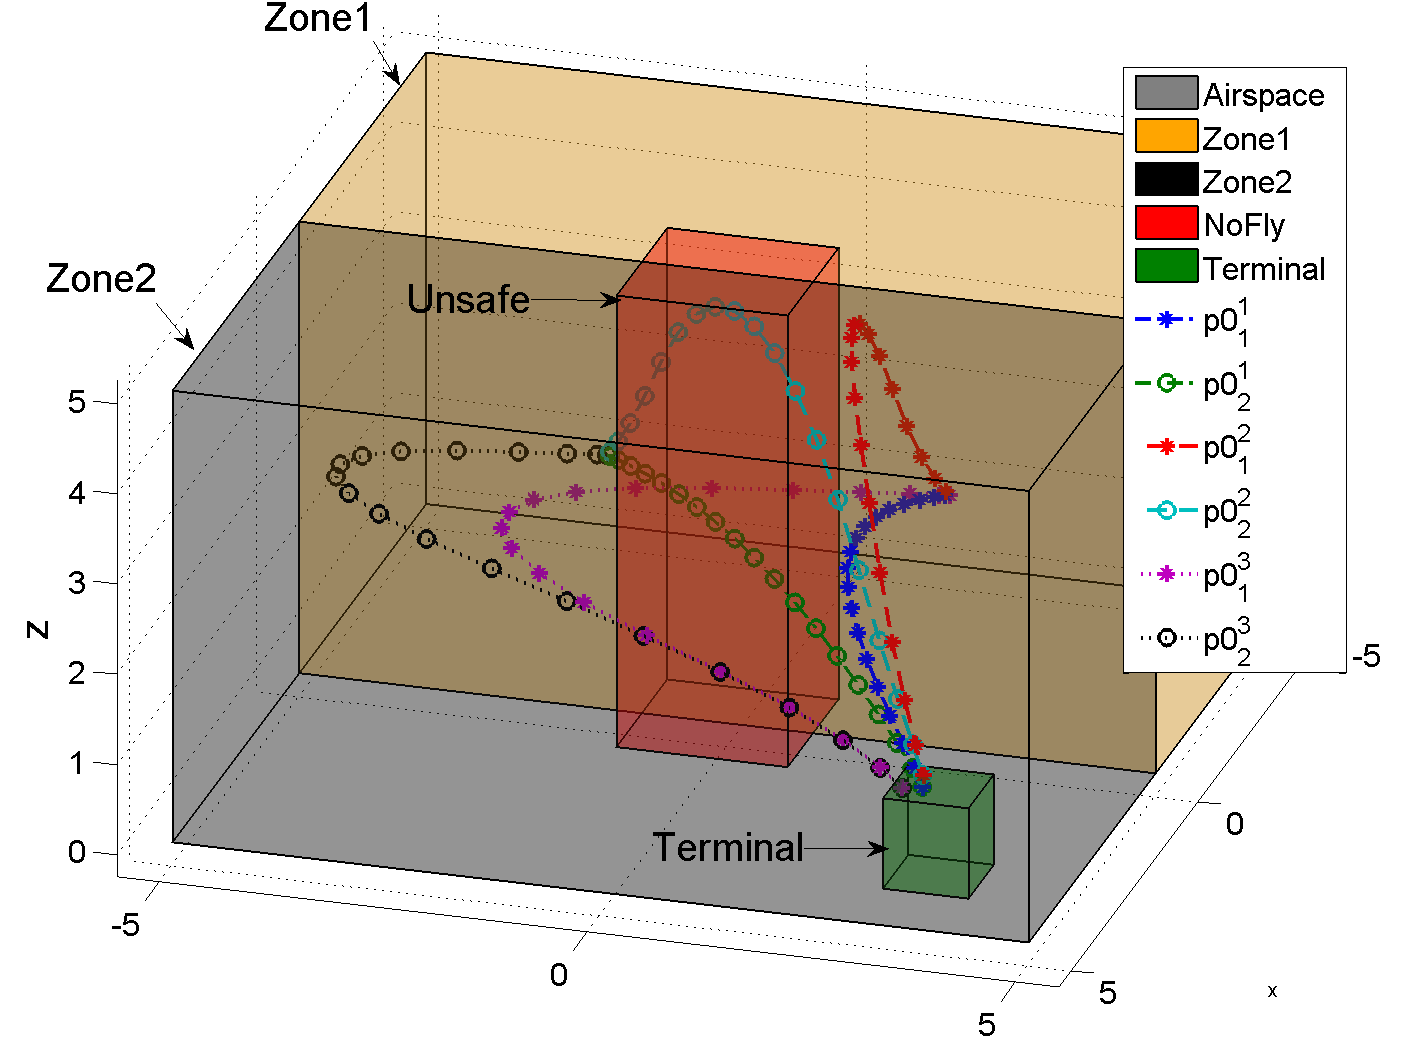
\includegraphics[width=0.49\textwidth]{figures/QuadInitTrajs_scissored}
\caption{The airspace with the corresponding sets, and initial trajectories for the two quad-rotors. Note, all 3 initial trajectories violate the specification. Here, $p0_{i}^j$ refers to the positions of the $i^{th}$ initial trajectory for the $j^{th}$ quadrotor.}
\label{fig:quad_init}
\end{figure}

\begin{figure}[t]
\centering
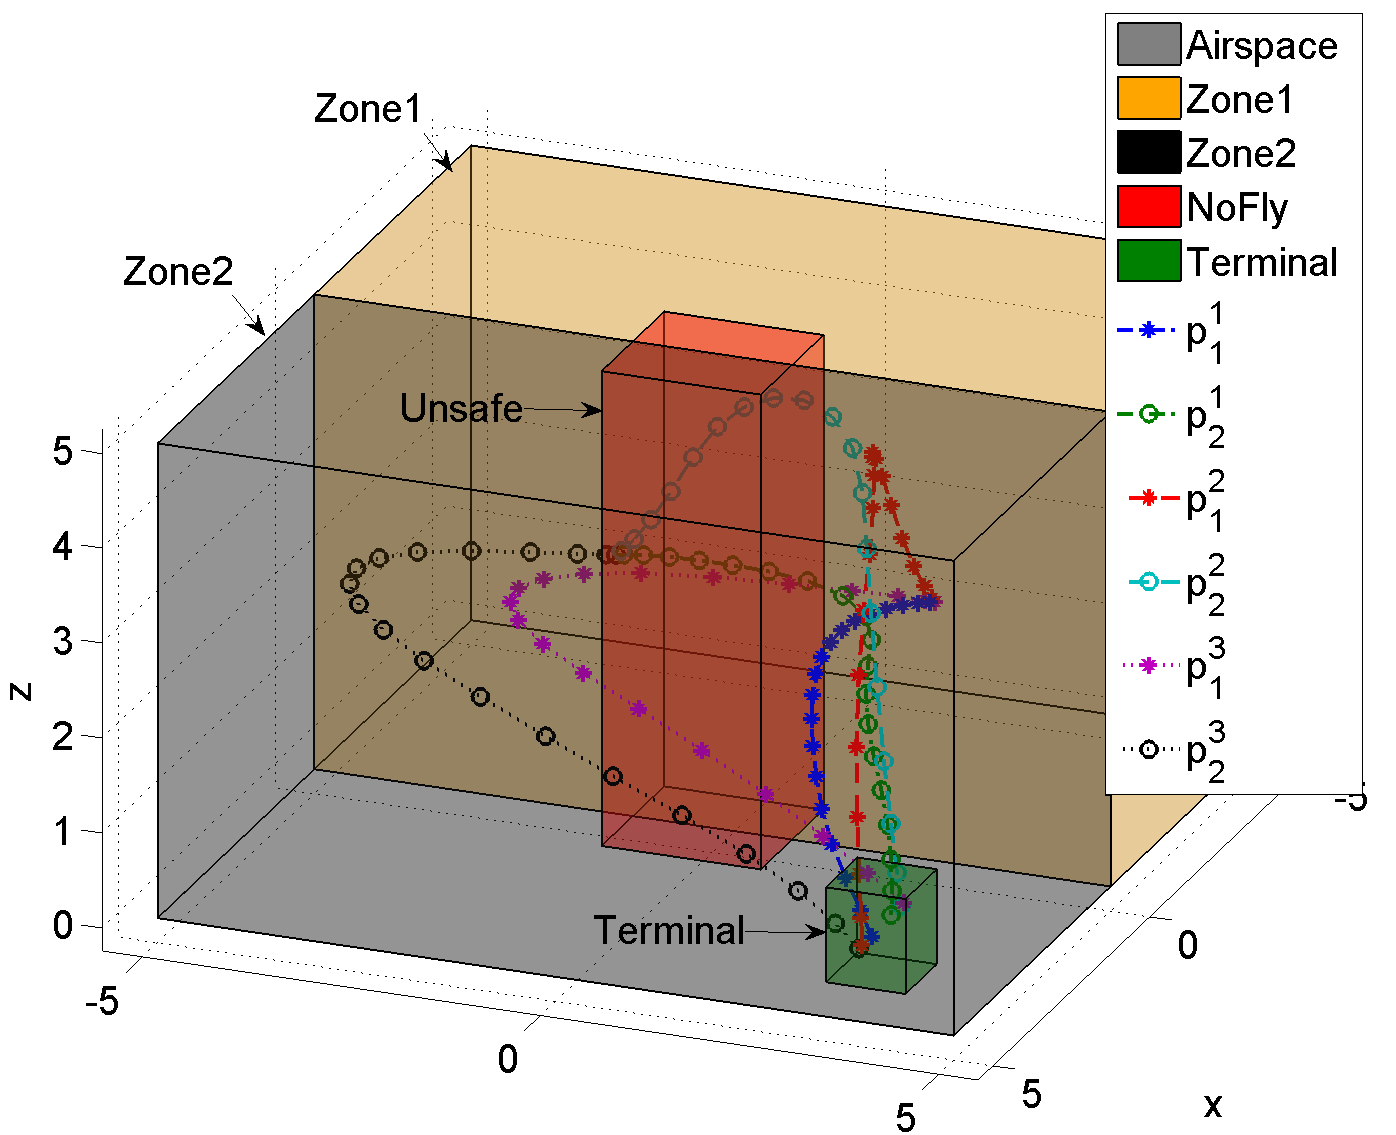
\includegraphics[width=0.49\textwidth]{figures/QuadTrajs_scissored}
\caption{ Trajectories obtained via SQP on smooth robustness, with three different initial trajectories acting as initial solutions for the SQP. Note, all 3 trajectories satisfy $\Psi$. Here, $p_{i}^j$ refers to the positions of the $i^{th}$ initial trajectory for the $j^{th}$ quadrotor.}
\label{fig:quad_ssqp}
\end{figure}

%\todo[inline]{%Start by motivating the example as something more than a dumb system. E.g. "Air traffic control offers many opportunities for automation to allow a more efficient and safer landing patterns. The constraints of air traffic control are complex and contain many safety rules. In this example we express these rules in MTL and demonstrate how the smoothed robustness is used to generate control strategies for safely and robustly landing two quadrotors. The proposed approach outperforms Simulated Annealing and gradient descent on %the non-smooth robustness."	Then you give the details below}
%1. We take a quad-rotor model with linearized dynamics around hover, similar to those used in \cite{}. The case study involves centralized control of two quad-rotors, with operational objectives given as an MTL specification, and a constrained air-space.

%1.b. Give model, constraints, specification. Shrinking horizon (fixing history) approach applicable (cite Vasu paper)

%2. With the given specification, standard control approaches involving polyhedral constraints are hard to apply because of the temporal aspect of the eventually operator involved. While the two (if-then) altitude rules in the specification can be coded as polyhedral constraints on the set, it would result in a non-convex constraint set for positions. Similarly, the minimum distance between two quad-rotors can also be moved to the constraints but would result in another non-convex constraint if we choose to do so. In our formulation, the non-convexity remains in the cost-function while the constraints are linear.

%3. For simulation purposes, we use obtain 3 initial trajectories (via solving different linear programs) from the given initial state to the terminal (landing) set. These three trajectories, each of which has negative robustness (i.e. does not satisfy the given specification), serve as three different initial solutions to A) Our approach B) SQP using the actual robustness function as the cost, C) Simulated Annealing with the actual robustness function as the cost. This multi-start approach can be used in practice when there is a fast initial trajectory generator available.

%3.b. parameters for simulation annealing and citation for it.

%4. Fig shows the initial trajectories for both the quadrotors in the given air-space. Fig. shows the three trajectories obtained after applying our control method, with the three initial trajectories as starting points for the optimization, respectively. 

%5. Table shows for the three trajectories, initial robustness, robustness for trajectory obtained via the three methods (and the approximate robustness when applicable). In addition, we also tested out simulated annealing with the smooth robustness function in the cost (with the first initial trajectory), resulting in a trajectory with a final cost of blah (approximate robustness of blah).
